\documentclass[a4paper]{article}
\usepackage[utf8]{inputenc}
\usepackage{amsmath}
\usepackage{amsfonts}
\usepackage{tikz}
\usepackage{tkz-euclide}
\usepackage{graphicx}
\graphicspath{ {./images/} }
\pagenumbering{gobble}

\begin{document}

\begin{center}
        \section*{Maths Problems Set 3 (17 January 2020)}
\end{center}

\begin{enumerate}
    \item
    Elves have incredible depth perception and can extremely accurately judge distances to objects. Ellie the elf is $2$ metres tall and on a pleasant stroll, sees a field of grass pass over the horizon $8000 \sqrt{\frac{2}{5}}$ metres away. Find the radius of the Earth.

    \item
    Peter and Sara are gnomes. Peter and Sara share a grandmother. Every 12 days Peter visits his grandmother. Every 30 days Sara visits her grandmother. Given that they sometimes visit on sequential days, do they ever visit on the same day?
    
    \item
    Prove the following:
    \begin{enumerate}
        \item $\sin^2 x + \cos^2 x = 1$
        \item $\sin(x + \frac{\pi}{2}) = \cos(x)$
        \item $\sin(x + a) = \sin (x) \cos (a) + \sin (a) \cos (x)$
    \end{enumerate}
    
    \item
    The city of Königsberg is situated on a river, with two islands in the river and seven bridges joining the two sides of the city and the islands as shown in the diagram below. Is it possible to walk across each bridge exactly once?
    
    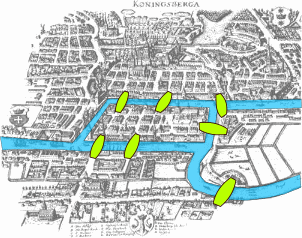
\includegraphics[scale=0.5]{konigsberg_bridges.png}
    
    \textit{Image credit: Bogdan Giuşcă - Public domain (PD) licensed under CC BY-SA 3.0}
    
    \item
    An empty cone has height $h$ metres and radius $r$ metres. Water is being poured into the cone at a rate of 3 cubic metres per second and no water drips out of the cone. Find the rate of increase of the height of the water

    \item
    Consider some number $n$. Take the sum of the digits of $n$. Let this sum now be the new value of $n$. Repeat this until the value of $n$ is less than 10. Show that if the final value of $n$ is 9, then the original value of $n$ was a multiple of 9, otherwise the final value of $n$ is equal to the remainder after the original value of $n$ is divided by 9.
    
    \item
    A particle is launched from height $h$ metres at an angle of $\theta$ with an initial velocity of $u$ metres per second. Given that it lands at an angle of $\frac{\pi}{4}$ above the horizontal, find an expression for $\theta$ in terms of $h$ and $u$.
    
    \item
    Prove Heron's formula, which states that the area $A$ of a triangle with sides $a$, $b$, and $c$, and semiperimeter $s$ is given by $A = \sqrt{s(s-a)(s-b)(s-c)}$. The semiperimeter $s$ is given by $\frac{a+b+c}{2}$.
    
    \item
    Evaluate $\int^{\frac{\pi}{3}}_{\frac{\pi}{6}} (\frac{\sin x}{x})^2 \mathrm{d}x - \int^{\frac{\pi}{3}}_{\frac{\pi}{6}} \frac{\sin 2x}{x} \mathrm{d}x$
    
    \item
    A real-valued function $f(x)$ is defined for all values of $x$ where $0 \leq x \leq 1$ and has a single turning point in this domain. It is a "black box" in that you can't see the graph of the function (and therefore can't take the derivative, etc.). The only thing you can do is evaluate the function at any value of $x$ in the given domain. 
    
    How accurately can you determine the x coordinate of the function's turning point by evaluating the function at most 10 times? What about $n$ times?
    
    
    
    \item
    Find the derivative and the integral of $\arcsin x$ (i.e. $\sin ^{-1} x$) with respect to $x$.
    
    \item
    Under what conditions on $a$, $b$ and $n$ does there exist at least one solution for for $x$ to the equation $ax = b \text{ (mod } n\text{)}$?
    
    \item
    There's a tank containing 10 litres of alcohol and 10 litres of water. Water is poured into the tank at a rate of 5 litres per minute, and the contents of the tank is poured out at a rate of 5 litres per minute. Assuming the liquids instantaneously mix and have uniform concentrations, find the time until the alcohol content is 0.2 litres.
    
    \item
    There are T bowls each containing some number of stones. Two players take turns removing 1, 2 or 3 stones from a pot of their choice. The player who takes the last stone from the last pot wins. Given that for any initial configuration one of the players has a forced win. Produce a strategy such that the player with the winning position can always force a win.
    
    \item
    Owen likes to play with stones and jars. Currently he has a red jar, a blue jar and a pile of 100 pebbles. Initially both jars are empty. A move consists of moving a pebble from the pile into one of the jars or returning a pebble from one of the jars to the pile.
    
    The numbers of pebbles in the red and blue jars determine the state of the game. The following conditions must be satisfied:
    
    \begin{enumerate}
        \item The red jar may never contain fewer pebbles than the blue jar
        \item The game may never be returned to a previous state
    \end{enumerate}
    
    \item
    Prove that for all prime numbers $p$, $(p-1)! + 1$ is divisible by $p$.
    
    
    
    
    
    
\end{enumerate}



\end{document}
